\graphicspath{{figures/appendix-error-propgate/}}

\chapter{速率系数不确定性传递函数的推导}
\label{appendix:error-propagate}

普通激发态(如 SUNIST 使用的 $n=4$ 能级)具有可以用来进行谱线诊断的谱线辐射,碰撞辐射模型对这些能级的计算精度是我们所主要关注的。因此,在速率系数不确定性函数的推导过程中,我们主要关注这些激发态能级的数密度。为了简化问题,在所有的感兴趣能级产生过程中,考虑同时只有其中某一个过程 $j\to p$ 的速率系数 $C_{jp}$ 具有不确定性\cite{Andrew2000PPCFSensitivity},研究其对感兴趣能级粒子数密度 $N_p$ 引起的相对误差。

对能级主要产生过程的分析我们可以得到,对于普通激发态能级,无论是电子碰撞复合产生过程,还是电离过程的数密度损失速率,都不足以超过其产生或损失总粒子数速率。所以,对于准稳态情况下的等离子体,$p$ 能级离子的总产生速率与总损失速率相等,则:
\begin{equation}
N_{\rm e}\sum_{i\ne p}C_{ip}N_i=N_{\rm e}N_p\sum_{i\ne p}C_{pi}+N_p\sum_{i<p}A_{pi}
\label{eq:appendix:error:rateequation}
\end{equation}
其中 $i$ 表示与 $p$ 能级发生电子碰撞激发、退激发或自发辐射过程的能级。$C_{ip}$、$C_{pi}$ 与 $A_{pi}$ 分别为 $p$ 能级的电子碰撞产生,损失与自发辐射速率系数。而电子密度、$i$ 能级与 $p$ 能级的粒子数密度分别记为 $N_{\rm e}$、$N_i$ 与 $N_p$。

从式 (\ref{eq:appendix:error:rateequation}) 可以解出 $N_p$:
\begin{equation}
N_p=\frac{N_{\rm e}\sum_{i\ne p}C_{ip}N_i}{N_{\rm e}\sum_{i\ne p}C_{pi}+\sum_{i<p}A_{pi}}
\label{eq:appendix:error:Np}
\end{equation}
这里,对于速率系数不确定性引起的 $N_p$ 相对误差,我们计入最大估计值\cite{YuChangxuan:book}:
\begin{eqnarray}
s_{N_p}=\frac{{\rm d}N_p}{N_p}& = &s\left(N_{\rm e}\sum_{i\ne p}C_{ip}N_i\right) + s\left(N_{\rm e}\sum_{i\ne p}C_{pi}+\sum_{i<p}A_{pi}\right)% \nonumber \\
% & = & \frac{}{} + \frac{}{}
\label{eq:appendix:error:EqOrig}
\end{eqnarray}
对于 $n=4$ 普通激发态,自发辐射能级产生或损失过程的速率小于总产生或损失速率的 $10\%$。同时,自发辐射速率系数可以精确得到\cite{NISTdatabase}。在式 (\ref{eq:appendix:error:EqOrig}) 右侧第二项中,忽略自发辐射过程的影响,则
\begin{eqnarray}
s_{N_p}& = &s\left(N_{\rm e}\sum_{i\ne p}C_{ip}N_i\right) + s\left(N_{\rm e}\sum_{i\ne p}C_{pi}\right) \nonumber\\
            & \simeq & \frac{{\rm d}F_{p,{\rm in}}}{F_{p,{\rm in}}} + \frac{{\rm d}F_{p,{\rm out}}}{F_{p,{\rm out}}}
\label{eq:appendix:error:EqIgnoreAqi}
\end{eqnarray}
其中 $F_{p,{\rm in}}=N_{\rm e}\sum C_{ip}N_i$ 与 $F_{p,{\rm out}}=N_{\rm e}N_p\sum C_{pi}$ 分别为 $p$ 能级的电子碰撞产生与损失总速率。根据精细平衡\cite{Lieberman2005-book}原则,认为电子碰撞激发与退激发具有相同的相对误差是合理的。则 $N_p$ 的相对误差可以写为:
\begin{eqnarray}
s_{N_p} \simeq 2\left(\frac{{\rm d}F_{p,{\rm in}}}{F_{p,{\rm in}}}\right)
\simeq 2\left(\frac{{\rm d}F_{p,{\rm out}}}{F_{p,{\rm out}}}\right)
\label{eq:appendix:error:EqFinal}
\end{eqnarray}
为了简化,此时仅考虑 $j\to p$ 过程的速率系数具有为 $s(C_{jp})={\rm d}C_{jp}/C_{jp}$ 的不确定性\cite{Andrew2000PPCFSensitivity},则 $p$ 能级的总产生速率相对误差为:
\begin{eqnarray}
{\rm d}F_{p,{\rm in}}={\rm d}f_{jp}&=&{\rm d}\left(N_{\rm e}N_jC_{jp}\right)\nonumber\\
&=&N_{\rm e}C_{jp}N_j\frac{{\rm d}C_{jp}}{C_{jp}}+N_{\rm e}C_{jp}N_j\frac{{\rm d}N_j}{N_j}\nonumber\\
&=&f_{jp}s\left(C_{jp}\right)+f_{jp}s\left(N_j\right)
\label{eq:appendix:error:dFin}
\end{eqnarray}
其中 $j\to p$ 过程的粒子反应速率记为 $f_{jp}$。根据式 (\ref{eq:appendix:error:EqFinal}),$s(N_j)$ 可以重写为
\begin{eqnarray}
s(N_j)\simeq 2\left(\frac{{\rm d}F_{j,{\rm out}}}{F_{j,{\rm out}}}\right)
\label{eq:appendix:error:sigmaNjOrig}
\end{eqnarray}
碰撞辐射模型的反应速率方程处于准稳态,则 $p$ 能级的粒子数总产生速率与总损失速率相等,所以
\begin{eqnarray}
F_{j,{\rm out}}&=&F_{j,{\rm in}}
\label{eq:appendix:error:FjinANDdFjin}
\end{eqnarray}
当速率系数的不确定性引起粒子数速率变化时,则有
\begin{eqnarray}
{\rm d}F_{j,{\rm out}}&\simeq&{\rm d}f_{jp}
\label{eq:appendix:error:dFjinANDdFjin}
\end{eqnarray}
那么式 (\ref{eq:appendix:error:sigmaNjOrig}) 即可以写为:
\begin{eqnarray}
s(N_j)\simeq 2\left(\frac{{\rm d}f_{jp}}{F_{j,{\rm in}}}\right)
\label{eq:appendix:error:sigmaNj}
\end{eqnarray}
将式 (\ref{eq:appendix:error:sigmaNj}) 代入式 (\ref{eq:appendix:error:dFin}),可以得到:
\begin{eqnarray}
{\rm d}f_{jp}=f_{jp}s\left(C_{jp}\right)+2f_{jp}\left(\frac{{\rm d}f_{jp}}{F_{j,{\rm in}}}\right)
\label{eq:appendix:error:dfjpEq}
\end{eqnarray}
则 ${\rm d}f_{jp}$ 可以简化为:
\begin{eqnarray}
{\rm d}f_{jp}=\left(1-\frac{2}{F_{j,{\rm in}}}\right)^{-1}f_{jp}s(C_{jp})
\label{eq:appendix:error:dfjp}
\end{eqnarray}
根据式 (\ref{eq:appendix:error:EqFinal})、(\ref{eq:appendix:error:dFin}) 与 (\ref{eq:appendix:error:dfjp}),我们可以得到速率系数不确定性 $s(C_{jp})$ 引起 $p$ 激发态能级粒子数 $N_p$ 的相对误差 $s_{N_p}$ 为
\begin{eqnarray}
s_{N_p}=E_{jp}s(C_{jp})=2\left(1-\frac{2}{F_{j,{\rm in}}}\right)^{-1}\frac{f_{jp}}{F_{p,{\rm in}}}s(C_{jp})
\label{eq:appendix:error:Propagation}
\end{eqnarray}
其中
\begin{eqnarray}
E_{jp}=2\left(1-\frac{2}{F_{j,{\rm in}}}\right)^{-1}\frac{f_{jp}}{F_{p,{\rm in}}}
\simeq 2\frac{f_{jp}}{F_{p,{\rm in}}}
\label{eq:appendix:error:PropagationCoeff}
\end{eqnarray}
为速率系数不确定性传递函数(the uncertainty propagation coefficient)。$F_{j,{\rm in}}$、$f_{jp}$ 与 $F_{p,{\rm in}}$ 可以从碰撞辐射模型的计算结果直接计算获得。在式(\ref{eq:appendix:error:PropagationCoeff}) 中假设
\begin{eqnarray}
F_{j,{\rm in}}\gg 2
\label{eq:appendix:error:FjinLargerThan2}
\end{eqnarray}
总是成立。

然而,式 (\ref{eq:appendix:error:Propagation}) 仅可用来计算与 $p$ 能级直接相关的反应过程速率系数不确定性的传递。具 SUNIST 参数的氦放电等离子体的电离度 $\sim 1$。其离子数含量非常之高,则 ${\rm He}^+$ 到基态能级 $1^1{\rm S}$ 的速率系数不确定性会通过基态的二级反应过程(secondary stepwise process)对感兴趣能级的粒子数产生影响。而 ${\rm He}^+$ 与 ${\rm He}^{2+}$ 之间的电离与复合过程速率系数则会通过三级反应过程,以及其他可以对基态能级粒子数总产生或消失速率产生影响的反应过程都会对对 $p$ 能级粒子数产生影响。

对于二级反应过程,$N_1$ 的粒子数密度会发生变化,而基态到 $p$ 的速率系数 $C_{1p}$ 不变。所以:
\begin{eqnarray}
{\rm d}f_{1p}=N_{\rm e}C_{1p}{\rm d}N_1\simeq N_{\rm e}C_{1p}N_1\frac{{\rm d}N_1}{N_1}=f_{1p}s(N_1)
\label{eq:appendix:error:secondary:df1p}
\end{eqnarray}
联立式 (\ref{eq:appendix:error:EqFinal})、(\ref{eq:appendix:error:dFin})、(\ref{eq:appendix:error:Propagation}) 与 (\ref{eq:appendix:error:secondary:df1p}),可以得到:
\begin{eqnarray}
s_{N_p}&=&2\frac{f_{1p}}{F_{p,{\rm in}}}s(N_1)
=2\frac{f_{1p}}{F_{p,{\rm in}}}E_{j1}s(C_{j1})\nonumber \\
&=&E_{j1p}s(C_{j1})
\label{eq:appendix:error:secondary:sigmaNp}
\end{eqnarray}
其中 $E_{j1}$ 与式 (\ref{eq:appendix:error:PropagationCoeff}) 具有相同的形式。

与上面二级反应过程相同的推导,$s(C_{{\rm He}^{2+}{\rm He}^+})$ 与 $s(C_{{\rm He}^+{\rm He}^{2+}})$ 到 $s_{N_p}$ 的传递可以分别写为:
\begin{eqnarray}
s_{N_p}&=&2^2\cdot\frac{f_{1p}}{F_{p,{\rm in}}}%s(N_1)
\cdot
\frac{f_{{\rm He}^+1}}{F_{1,{\rm in}}}
\cdot
E_{{\rm He}^{2+}{\rm He}^+}s(C_{{\rm He}^{2+}{\rm He}^+})\nonumber\\
&=&E_{{\rm He}^{2+}{\rm He}^+1p}s(C_{{\rm He}^{2+}{\rm He}^+})
\label{eq:appendix:error:HeII:sigmaNp}
\end{eqnarray}
与
\begin{eqnarray}
s_{N_p}&=&2^3\cdot\frac{f_{1p}}{F_{p,{\rm in}}}%s(N_1)
\cdot
\frac{f_{{\rm He}^+1}}{F_{1,{\rm in}}}
\cdot
\frac{f_{{\rm He}^{2+}{\rm He}^+}}{F_{{\rm He}^+,{\rm in}}}
\cdot
E_{{\rm He}^+{\rm He}^{2+}}s(C_{{\rm He}^+{\rm He}^{2+}})\nonumber\\
&=&E_{{\rm He}^+{\rm He}^{2+}{\rm He}^+1p}s(C_{{\rm He}^+{\rm He}^{2+}})
\label{eq:appendix:error:HeIII:sigmaNp}
\end{eqnarray}

最后,我们可以将速率系数不确定性通过 $i\to j\to\cdots\to q\to p$ 多级反应过程传递给 $s_{N_p}$ 的不确定性传递函数写为:
\begin{eqnarray}
E_{ij\cdots qp}=E_{qp}E_{.q}\cdots E_{j.}E_{i\to j}
\label{eq:appendix:error:MPDcoefficient}
\end{eqnarray}

图 \ref{fig:appendix:error-prop:1}--图 \ref{fig:appendix:error-prop:8} 分别为本工作使用的碰撞辐射模型中,多种反应速率系数的不确定性传递函数计算结果。

\begin{figure}%[H]
    \centering
    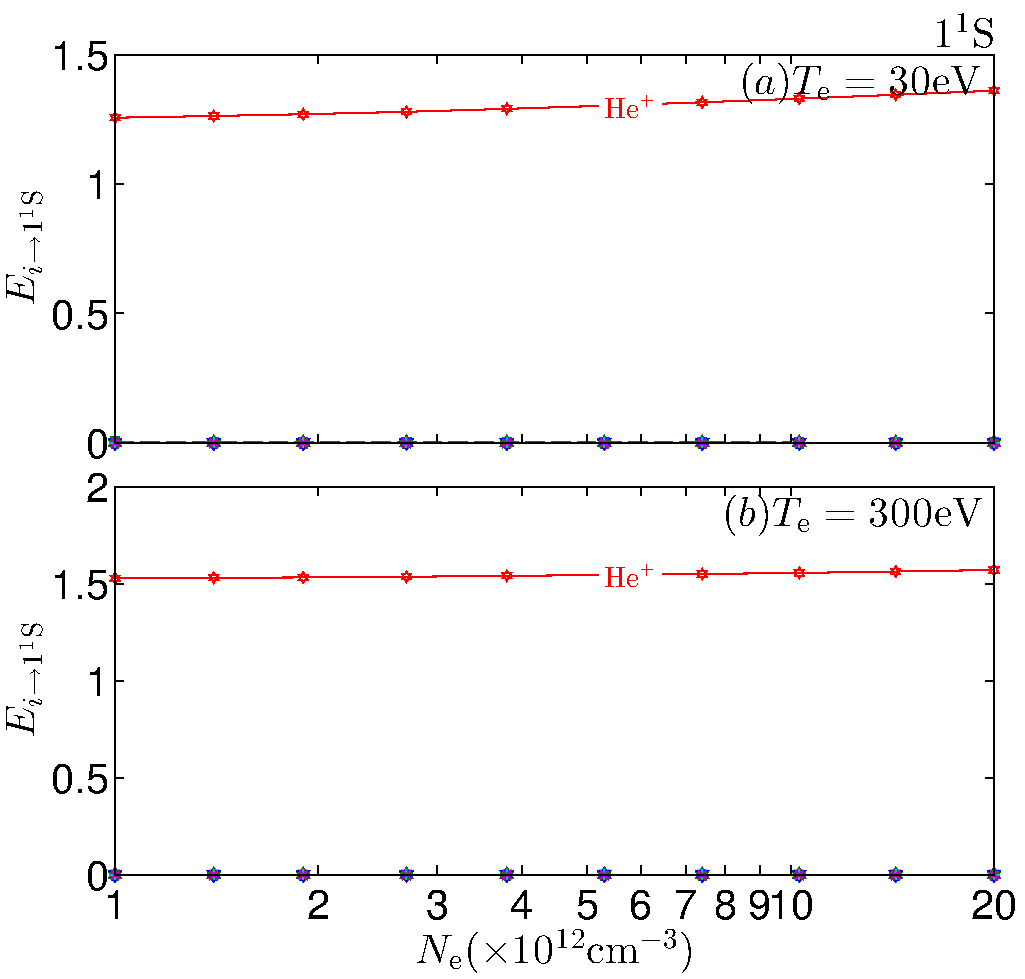
\includegraphics[width=0.6\textwidth]{11S-error-propagation-coefficient.pdf}
    \caption{所有能级至基态 $1^1{\rm S}$ 直接产生过程速率系数的不确定性传递函数}
    \label{fig:appendix:error-prop:1}
\end{figure}

\begin{figure}%[H]
    \centering
    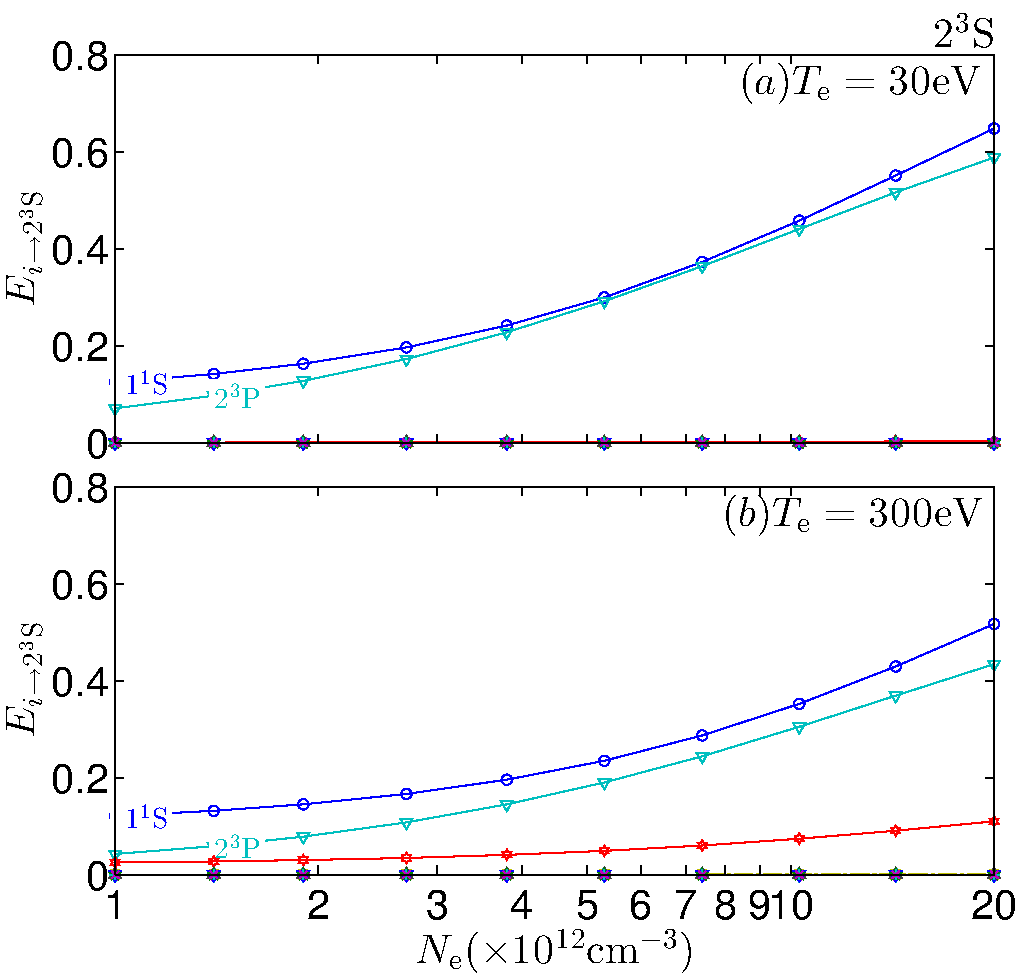
\includegraphics[width=0.6\textwidth]{23S-error-propagation-coefficient.pdf}
    \caption{所有能级至亚稳态 $2^3{\rm S}$ 直接产生过程速率系数的不确定性传递函数}
    \label{fig:appendix:error-prop:2}
\end{figure}

\begin{figure}%[H]
    \centering
    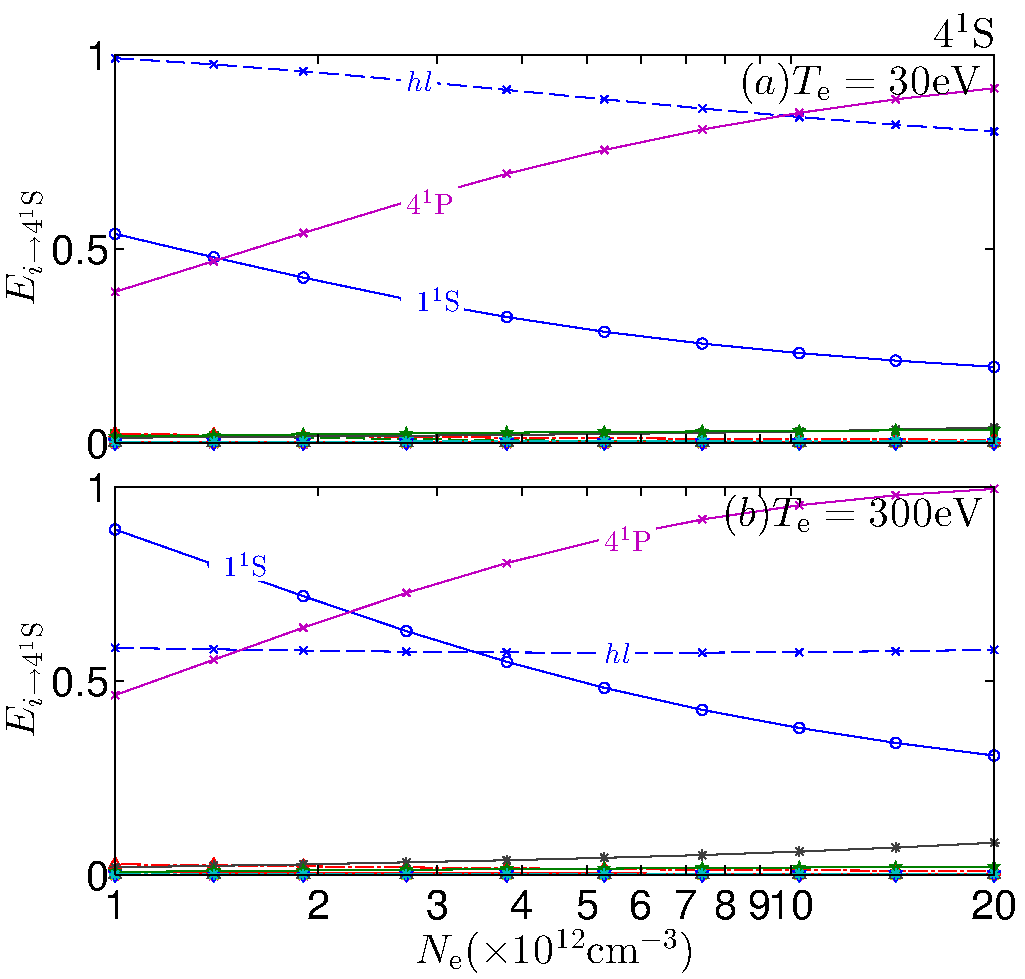
\includegraphics[width=0.6\textwidth]{41S-error-propagation-coefficient.pdf}
    \caption{所有能级至 $4^1{\rm S}$ 能级直接产生过程速率系数的不确定性传递函数}
    \label{fig:appendix:error-prop:3}
\end{figure}

\begin{figure}%[H]
    \centering
    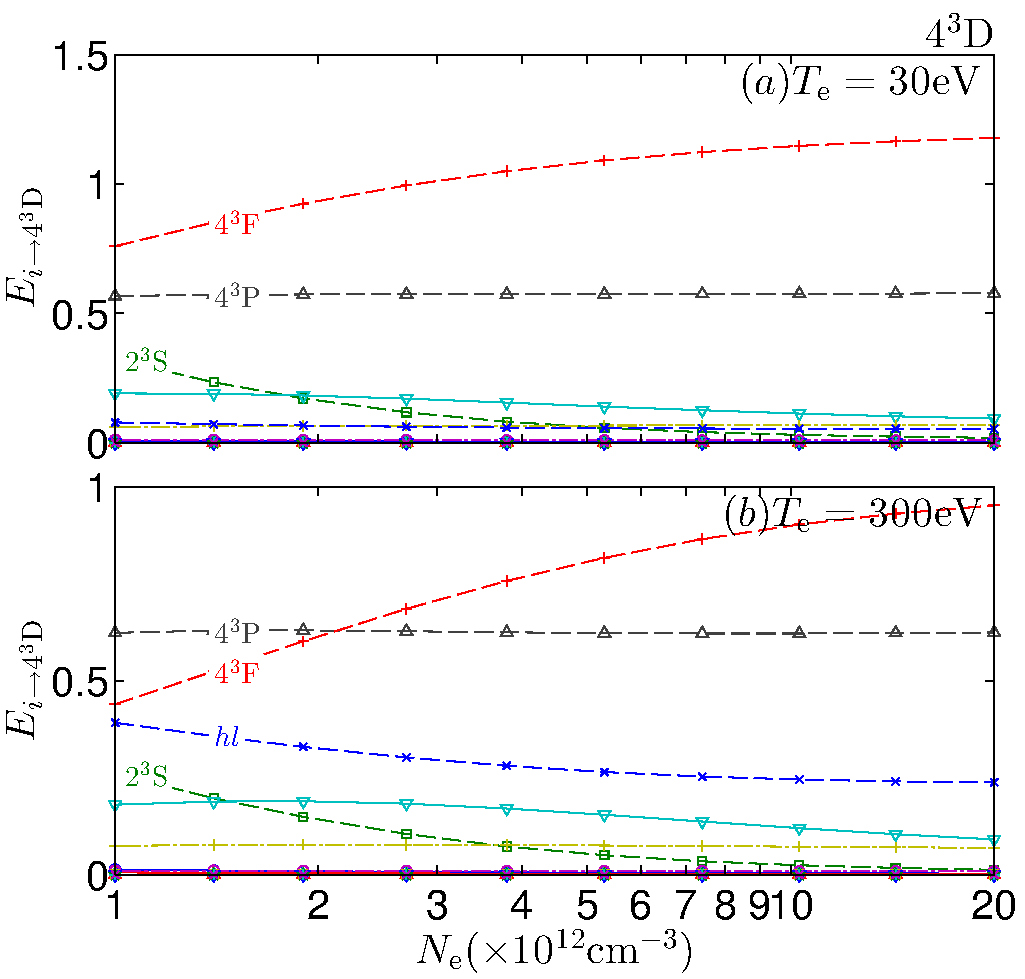
\includegraphics[width=0.6\textwidth]{43D-error-propagation-coefficient.pdf}
    \caption{所有能级至 $4^3{\rm D}$ 能级直接产生过程速率系数的不确定性传递函数}
    \label{fig:appendix:error-prop:4}
\end{figure}

\begin{figure}%[H]
    \centering
    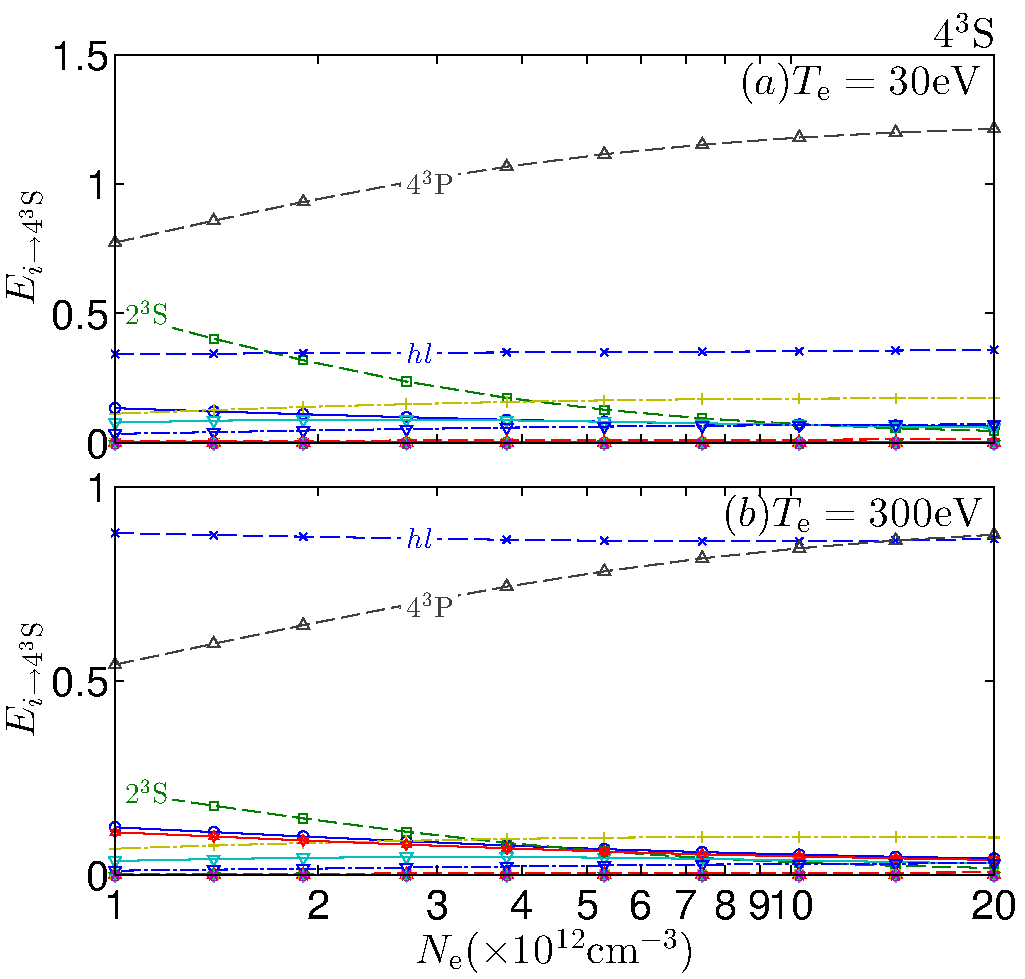
\includegraphics[width=0.6\textwidth]{43S-error-propagation-coefficient.pdf}
    \caption{所有能级至 $4^3{\rm S}$ 能级直接产生过程速率系数的不确定性传递函数}
    \label{fig:appendix:error-prop:5}
\end{figure}

\begin{figure}%[H]
    \centering
    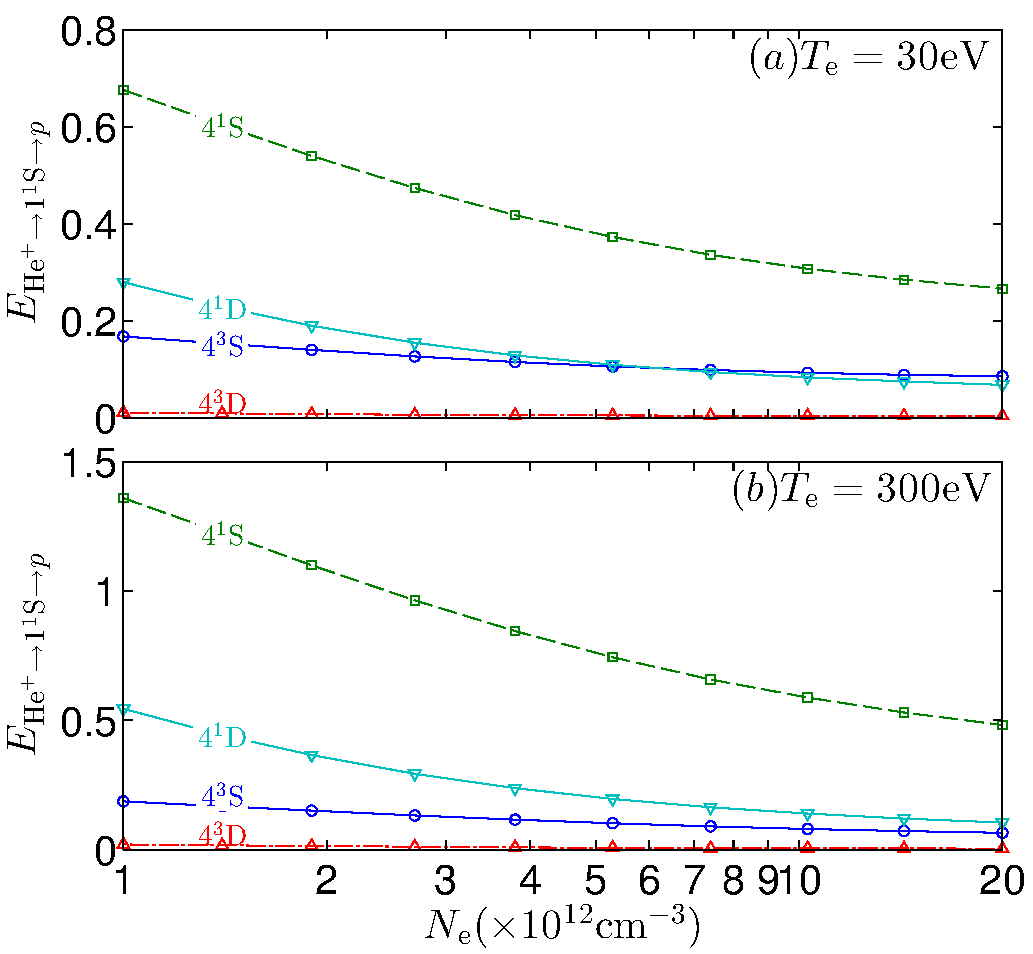
\includegraphics[width=0.6\textwidth]{HeII1p-error-propagation-coefficient.pdf}
    \caption{所有能级至 ${\rm He}^+$ 离子复合到基态能级 $1^1{\rm S}$ 的速率系数不确定性经二级反应过程至 $n=4$ 能级的传递函数}
    \label{fig:appendix:error-prop:6}
\end{figure}

\begin{figure}%[H]
    \centering
    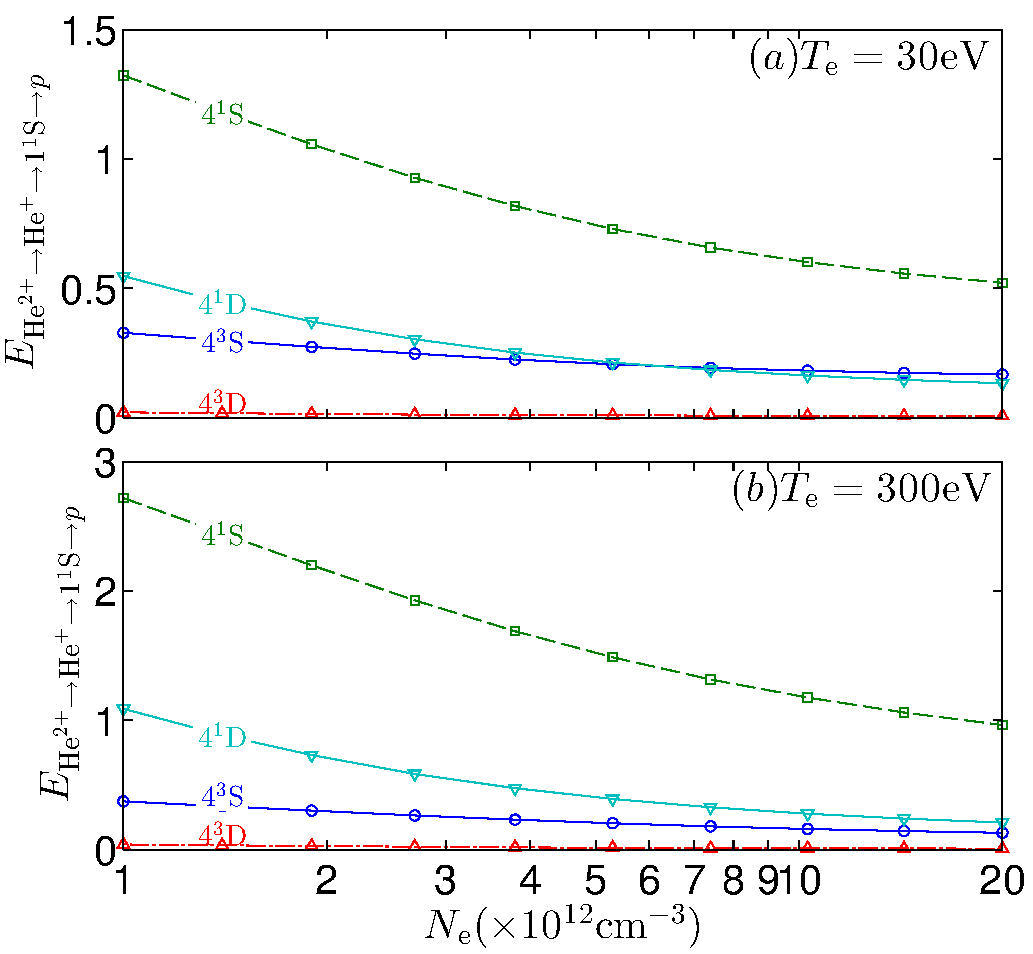
\includegraphics[width=0.6\textwidth]{HeIIIHeII1p-error-propagation-coefficient.pdf}
    \caption{${\rm He}^{2+}$ 离子复合到 ${\rm He}^+$ 的速率系数经三级级反应过程至 $n=4$ 能级的传递函数}
    \label{fig:appendix:error-prop:7}
\end{figure}

\begin{figure}%[H]
    \centering
    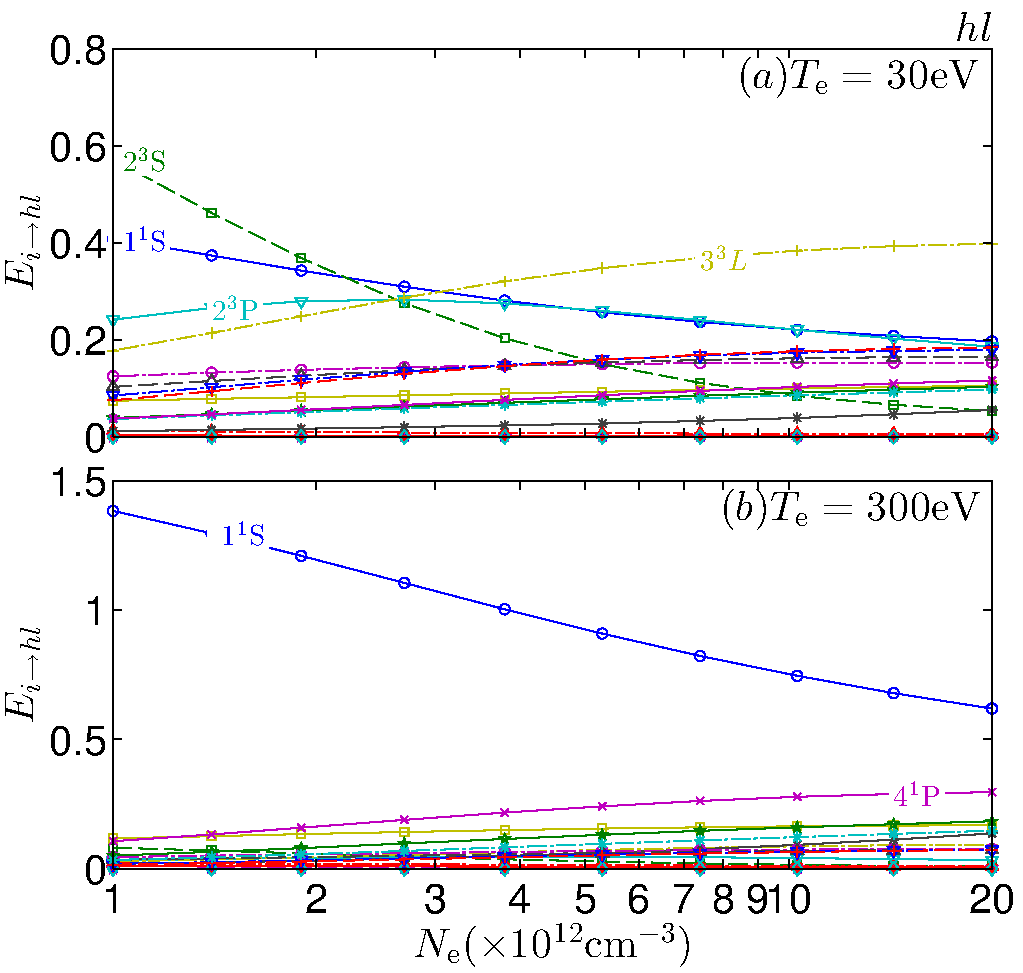
\includegraphics[width=0.6\textwidth]{hl-error-propagation-coefficient.pdf}
    \caption{其他能级至 $n\ge5$ 高能级 $hl$ 速率系数的传递函数}
    \label{fig:appendix:error-prop:8}
\end{figure}
